\documentclass[
    11pt,               % KOMA default
    a4paper,            % DIN A4
    %twoside,            % Zweiseitig
%     onside,
    headsepline,        % Linie unter der Kopfzeile
    foodsepline,        % Linie �ber Fussnote
    %automark,           % Kolumnentitel lebendig
    %pointlessnumbers,   % Keinen Punkt hinter die letzte Zahl
                        % eines Kapitels (auch bei Anhang)
%     openleft,           %
    %openright,
    cleardoubleplain,   %
    %abstracton,         %
    %idxtotoc,           % Index soll im Inhaltsverzeichnis auftauchen
    liststotoc,         %
    bibtotoc,           %
    %parskip            % parskip-, parskip*, parskip+
]%{scrreprt}
{article}

%\usepackage[latin1]{inputenc}
\usepackage[utf8]{inputenc}
\usepackage{ngerman}
\usepackage{graphicx}
\usepackage{subfigure}
\usepackage{float}
\usepackage{listings}
\usepackage{color}
\usepackage{tabularx}
\usepackage{hyperref}
\usepackage{tabu}
\usepackage{booktabs}
\usepackage[table]{xcolor}
\usepackage{url}
\usepackage{lmodern}
\usepackage{amsmath}
\usepackage{amsfonts}
\usepackage{amssymb}
\usepackage{enumitem}

% Definitions
\definecolor{mydarkblue}{rgb}{0.0,0.0,0.5}
\definecolor{mylightblue}{rgb}{0.85,0.85,0.85}
\definecolor{mylightgray}{rgb}{0.95,0.95,0.95}
\lstdefinelanguage{Spark}{
  keywords={type, new, record, function, return, null, procedure, is, array, if, in, of, do, range, case, subtype, others},
  keywordstyle=\color{blue}\bfseries,
  ndkeywords={Integer,Boolean,String,Character,True,False,Float,Positive,Natural,Real},
  ndkeywordstyle=\color{red}\bfseries,
  identifierstyle=\color{black},
  sensitive=false,
  comment=[l]{--},
  morecomment=[s]{/*}{*/},
  commentstyle=\color{purple}\ttfamily,
  stringstyle=\color{red}\ttfamily,
  morestring=[b]"
}
\lstset{
   language=Spark,
   backgroundcolor=\color{lightgray},
   extendedchars=true,
   basicstyle=\footnotesize\ttfamily,
   showstringspaces=false,
   showspaces=false,
   numbers=left,
   numberstyle=\footnotesize,
   numbersep=9pt,
   tabsize=2,
   breaklines=true,
   showtabs=false,
   captionpos=b
}
\newcommand{\HRule}{\rule{\linewidth}{0.4mm}}

\clubpenalty=10000
\widowpenalty=10000

\begin{document}

%\newpage
\pagestyle{empty}
\begin{center}
	
\includegraphics[scale=0.8]{hszg_logo.png}\\
	\vspace*{2cm}
	%\Large
	%\textbf{Fakultät}\\
	%\textbf{Elektrotechnik und Informatik}\\
	%\vspace*{2cm}
	\Huge
	\textbf{Belegarbeit}\\
	\Large
	\vspace*{2cm}
	\textbf{SPARK}\\
	\vspace*{1cm}
	
	\vfill
	\normalsize
	\newcolumntype{x}[1]{>{\raggedleft\arraybackslash\hspace{0pt}}p{#1}}
	\begin{tabular}{x{6cm}p{7.5cm}}
		\rule{0mm}{5ex}Riedel, Robert & {Matr.-Nr.:} 202349\\
		\rule{0mm}{5ex}Zoeke, Robert & {Matr.-Nr.:} 200074\\

		\rule{0mm}{5ex}\textbf{Abgabedatum:} & x.x.2015 \\ 
	\end{tabular} 
\end{center}
\include{abstract}
\pdfbookmark{\contentsname}{toc}\tableofcontents
\thispagestyle{empty}

\newpage
\pagestyle{empty}
\listoffigures

\newpage
\listoftables

\newpage
\pagestyle{plain}
\setcounter{section}{0}
\pagenumbering{arabic}

\section{Einleitung}
Software ist in unserer heutigen Gesellschaft nicht mehr wegzudenken. Die meisten Bereiche unseres Lebens werden von einer Software erfasst, bzw. gesteuert. Viele dieser Softwaresysteme sind unkritisch. So kann ein Officeprogramm abstürzen, ohne dass dadurch Menschenleben gefährdet werden. Wenn der Nutzer regelmäßig speichert, hat solch ein Absturz nur minimale Auswirkungen. Wenn jedoch die ABS Steuerung eines Autos für kurze Zeit versagt, kann dies schwerwiegende Folgen haben.
Für kritische Umgebungen gibt es spezielle Sprachen, wie z.B. \textbf{Ada}.
Ada erfüllt alle Kriterien einer solchen Sprache\footnote{Quelle: Vorlesungefolien Böhm SS2015}
\begin{itemize}
\setlength\itemsep{0.5em}
\item Portierbarkeit
\item Einsatz moderner SW-Engineering Methoden
\item Multitasking
\item Schnittstellen zu anderen Programmiersprachen
\item Funktionsfähigkeit \begin{enumerate}
\item Sichere Datentypen
\item Willkürliche Sprünge
\item Speicherüberschreibungen
\end{enumerate}
\item Verfügbarkeit
\begin{enumerate}
\item Logische Gültigkeit
\item Initialisierungsfehler
\item Ausdrucksauswertungsfehler
\item Leistung
\end{enumerate}
\item Zuverlässigkeit
\begin{enumerate}
\item Mehrfache Referenzen
\item Seiteneffekte durch Unterprogramme
\item Speicherüberwachung
\end{enumerate}
\item Verständlichkeit
\item Testbarkeit, Verifizierbarkeit
\item Wiederherstellbarkeit
\item Wartbarkeit, Erweiterbarkeit und Wiederverwendbarkeit
\end{itemize}

Für spezielle Anwendungsfälle gibt es das Subset von Ada \textbf{Spark}. Spark ist eine Teilsprache von Ada, d.h. es wurden einige Konzepte von Ada weggelassen, was zu einem stark eingeschränkten Sprachkern geführt hat.
In dieser Arbeit werden wir die sprachlichen Unterschiede zu Ada erläutern und anschließend auf die speziellen Analysetools eingehen, die Spark zur Verfügung stellt. Sofern nicht anders ausgewiesen ist unsere Quelle das Buch High Integrity Software The Spark Approach to Safety and Security von John Barnes.
\section{Sprache}
\subsection{Typenmodell}
\label{subsec:Typenmodell}
\subsubsection{Objekte}
\label{subsubsec:Objekte}
Objekte sind Instanzen, die Werte eines gegebenen Typs enthalten. Das umfasst sowohl Objekte im Sinn der objektorientierten Programmierung wie auch einfache Instanzen. Objekte werden allgemein durch Objektdeklarationen deklariert, aber auch formale Parameter von Unterprogrammen und loop-Parameter werden als Objekte behandelt. Ebenso sind Komponenten von Objekten auch Objekte.\\
Objekte sind entweder Variablen oder Konstanten. Konstanten müssen initialisiert werden und auch der Wert von Variablen muss zur Zeit der Kompilierung bekannt sein.\\
\begin{lstlisting}[caption={Beispiele für einfache Objekte in Spark}, label=spark:einfacheObjekte]
Count, Sum: Integer;
Sorted: Boolean := False;
Limit: constant Integer := 10_1000;
Level: constant Float := 3.5;
\end{lstlisting}


Es ist nicht möglich bei der Objektdeklaration einen expliziten Constraint anzugeben. Das heißt, dass der (Sub-)Typ eines Objektes immer mit dem Schlüsselwort \texttt{subtype} und nicht nur durch einen Subtypindikator festgelegt wird.

\begin{lstlisting}[caption={Deklaration gültig in Ada, aber unzulässig in Spark}, label=ada:falscheDeklarationinAda]
I, J, K: Integer range 1 .. 10;
\end{lstlisting}

\begin{lstlisting}[caption={korrekte Deklaration in Spark}, label=spark:korrekteDeklarationinSpark]
subtype Index is Integer range 1 .. 10;
I, J, K: index;
\end{lstlisting}


Listing~\ref{spark:korrekteDeklarationinSpark} zeigt, dass alle Objekte in \texttt{Spark} benannte Subtypen haben müssen(außer loop-Parametern).

%TODO later layoutcheck for free page
\newpage

\subsubsection{Typen und Subtypen}
\label{subsubsec:TypenUndSubtypen}

\begin{figure}[h!]
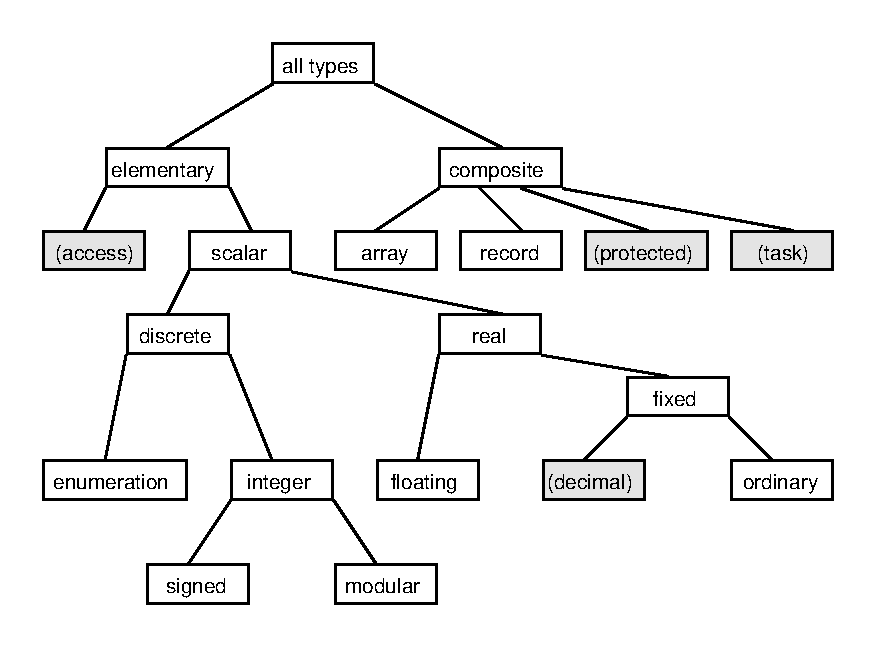
\includegraphics[width=\textwidth{}]{images/typeHierarchy.pdf}
\label{fig:typeHierarchy}
\caption{Hierarchie der Typen in Ada und Spark}
\end{figure}

Abbildung~\ref{fig:typeHierarchy} zeigt die verfügbaren Typen in \texttt{Ada} und mit grauer Hinterlegung bzw. in Klammern geschrieben die in \texttt{Spark} nicht verfügbaren Typen: \textit{access}, \textit{protected}, \textit{task} und \textit{decimal}.\\
Die in \texttt{Spark} vordefinierten Typen sind:\\
enumeration:
\begin{itemize}
	\item Boolean
	\item Character
\end{itemize}
fixed point type:
\begin{itemize}
	\item Duration
\end{itemize}
integer:
\begin{itemize}
	\item Integer
	\item Long\_Integer
\end{itemize}
float:
\begin{itemize}
	\item Float
	\item Long\_Float
\end{itemize}
array:
\begin{itemize}
	\item String
\end{itemize}

Weitere Typen können wie in \texttt{Ada} deklariert werden, jedoch mit gewissen Einschränkungen.\\
\textit{Ranges} müssen \textit{statisch} sein, also ihre Größe zur Kompilierung bekannt sein. Es können dazu also keine Variablen oder Funktionen verwendet werden. Da \textit{constraints} in \texttt{Spark} immer statisch sein müssen, sind auch ihre Attribute \textit{Last} und \textit{First} statisch und können verwendet werden(Listing~\ref{spark:Range constraint}).

\begin{lstlisting}[caption={Range constraint}, label=spark:Range constraint]
subtype Color is Colour range Colour'First .. Colour'Last;
\end{lstlisting}

Möchte man nur eine Umbenennung eines Typen vornehmen, so kann auch eine Kurzform verwendet werden(Listing~\ref{spark:Range constraint short}). Das ist aber nur für \textit{scalar}-Typen zulässig und nicht für \textit{private}-Typen.

\begin{lstlisting}[caption={Range constraint kurz}, label=spark:Range constraint short]
subtype Color is Colour;
\end{lstlisting}

Im Gegensatz zu \texttt{Ada} darf eine \textit{static range} in \texttt{Spark} niemal \textit{null} bzw. \textit{empty} sein, d.h. Die obere Grenze muss größer oder gleich der unteren sein(\textit{null ranges} in \textit{loops} sind erlaubt).

\begin{lstlisting}[caption={Typ des subtyps}, label=spark:Typ des subtyps]
type Colour is (White, Red, Yellow, Green, Blue, Brown);
subtype Rainbow is Colour range Red .. Blue;
R: Rainbow;
\end{lstlisting}

Zu Listing~\ref{spark:Typ des subtyps} ist wichtig, dass der Typ von \textit{R} immer noch \textit{Colour} ist.



\subsubsection{Enumaration Typen}
\label{subsubsec:EnumarationTypen}
Um die Mehrdeutigkeit zu reduzieren ist es in \texttt{Spark} nicht möglich \textit{literale} im selben \textit{scope} zu überladen. Listing~\ref{spark:literaleUeberladen} zeigt solch eine ungültige Überladung, welche in \texttt{Ada} möglich ist, in \textit{Spark} jedoch nicht möglich ist, da das \textit{literal} \textsc{Sun} in beiden Typen verwendet wird.

\begin{lstlisting}[caption={Literale überladen}, label=spark:literaleUeberladen]
type day is (Mon, Tue, Wed, Thu, Fri, Sat, Sun);
type SolarSystem is (Sun, Mercury, Venus, Earth);
\end{lstlisting}

Die aus \texttt{Ada} bekannten Vergleichsoperatoren und Attribute von \textit{enumerations} finden ihre normale Anwendung in Bezug auf ihre Reihenfolge bei der Deklaration. Sie beziehen sich aber auf den zu Grunde liegenden Typ. So ergibt \textsl{Rainbow'Succ(x)} das selbe wie \textsl{Colour'Succ(x)} auch wenn \textsl{x = blue}. Das führt dazu, dass keine eigenen character Typen deklariert werden können.\\
Der Typ \textit{Boolean} ist auch ein \textit{Enumaration} Typ, unterliegt in \texttt{Spark} aber besonderen Beschränkungen. Vergleichsoperatoren außer der (Un-)Gleihiet funktionieren nicht. Die Attribute \textit{Pred},\textit{Succ}, \textit{Pos} und \textit{Val} können nicht verwendet werden, aber \textit{First} und \textit{Last}. \textit{Boolean}s können als \textit{array index type} verwendet werden jedoch nicht als explizite \textit{range}. Verdeutlicht wird dies in Listing~\ref{spark:Boolean}.

\begin{lstlisting}[caption={Boolean}, label=spark:Boolean]
subtype ValveOpen is Boolean;  --erlaubt
subtype ValveOpen is Boolean range Boolean'First .. Boolean'Last; --falsch
subtype Always is Boolean range True .. True --falsch
\end{lstlisting}

Die Operationen \textit{and}, \textit{or}, \textit{xor} und \textit{not} haben ihre normale Bedeutung, wobei ein \textit{xor} einem \textit{/=} entspricht. 


\subsubsection{composite Typen}
\label{subsubsec:compositeTypen}
Es darf immer nur \textbf{ein} von einem \textit{tagged type} abgeleiteten Typen pro \textit{package} geben. Deswegen darf von den Deklarationen in Listing~\ref{spark:compositeTagged} immer nur eine je \textit{Package} stehen. Dadurch soll Überladung verhindert werden. Die entsprechenden Deklarationen können aber in Kindpaketen geschehen.

\begin{lstlisting}[caption={tagged types}, label=spark:compositeTagged]
type object is tagged
	record
		XCoord,YCoord: Float;
	end record;

type point is new Object with null record;

type Circle is new Object with
	record
		Radius: Float;
	end record;
\end{lstlisting}

\textit{Records} können, ebenso wie Objekte, keine \textit{constraints} enthalten. Ebenso können keine default-Werte vergeben werden. \textit{Records} in \texttt{Spark} sind daher recht einfach gestaltet und haben z.B. keine Diskriminanten.\\
\\
Auch \textit{Arrays} unterliegen den typischen Konventionen von \texttt{Spark}, dass jeder Typ benannt werden muss. Listing~\ref{spark:illegalArrays} zeigt in \texttt{Spark} ungültige Deklarationen von \textit{Arrays}, welche in Listing~\ref{spark:legalArrays} konform zu \texttt{Spark} gezeigt sind.

\begin{lstlisting}[caption={illegal Arrays}, label=spark:illegalArrays]
type Triple is array (1 .. 3) of Real;---falsch

UpperCaseTable: array(1 .. 10) of Character range 'A' .. 'Z';--falsch

NextLine:String(1 .. 80):--falsch
\end{lstlisting}
\begin{lstlisting}[caption={legal Arrays}, label=spark:legalArrays]
type Tuple is array (Integer range <>) of Real;
subtype TripleIndex is Integer range 1 .. 3;
subtype Triple is Tuple(TripelIndex);

subtype Index is Integer range 1 .. 10;
subtype CapitalLetter is Character range 'A' .. 'Z';
type UpperCaseArray is array (Index) of CapitalLetter;
UpperCaseTable: UpperCaseArray;

subtype LineIndex is Integer range 1 .. 80;
subtype Line is String(LineIndex);
NextLine: Line;
\end{lstlisting}

Alle \textit{constraints} in \texttt{Spark} sind \textit{statisch}, haben also \textit{statische Grenzen}, was dazu führt, dass in \texttt{Spark} keine Arrays deklariert werden können, deren Grenzen nicht zur Programmausführung bekannt sind.


\include{PackagesUndSichbarkeit}
\subsection{Kontroll- und Datenfluss}
\label{subsec:KontrollUndDatenfluss}
\textit{if}- und \textit{case}-Strukturen sind in \texttt{Spark} genauso wie in \texttt{Ada}. \textit{for}-Schleifen sind leicht anzupassen, s. Listing~\ref{spark:for-Schleifen}.
\begin{lstlisting}[caption={for-Schleifen}, label=spark:for-Schleifen]
for I in 1 .. 10 loop  --falsch

for I in Integer range 1 .. 10 loop
\end{lstlisting}

\textit{while}- und \textit{for}- Schleifen ebenso wie einfache \textit{loop}-Anweisungen können auch \textit{exit}-Anweisungen enthalten. Auch mehrere exit-Anweisungen in einem \textit{loop} werden immer alle ausgewertet.
\begin{lstlisting}[caption={exit in loop}, label=spark:exit in loop]
loop
	Get(CurrentCharacter);
	exit Search when CurrentCharacter = '*';
end loop Search;
\end{lstlisting}

\textit{return}-Anweisungen können in \texttt{Spark} nur in Funktionen verwendet werden und das auch nur exakt einmal am ende der Funktion. Es ist nicht möglich sie wie in \texttt{Ada} zum zurückkehren zum Prozeduraufruf zu verwenden.\\\


Es gibt in \texttt{Spark} keine \textit{Exception}, \textit{Labels}, \textit{Goto}-Anweisungen, \textit{Blöcke}. Unterprogramme können nicht rekursiv aufgerufen werden.
\section{Sprache}
\label{sec:Sprache}
\texttt{Spark} ist eine Teilmenge von \texttt{Ada}, welche besonders auf erhöhte Sicherheit bedacht ist. Aus diesem Grund werden einige Möglichkeiten von \texttt{Ada} beschnitten. Das übergeordnete Ziel ist es, eine statische Analyse des Codes zu ermöglichen. In erster Linie werden dazu Annotationen eingeführt, welche den Ada-Code ergänzen und Informationen für den Examiner(s. ~\ref{sec:examiner}) bereitstellen.

\subsection{Annotationen}
\label{subsec:Annotationen}
Zur Kompilierung von \texttt{Spark} wird ein \texttt{Ada}-Kompiler verwendet, das heißt jedes \textit{gültige} Programm in \texttt{Spark} ist auch in \texttt{Ada} gültig. Es gibt jedoch viele Dinge , die in \texttt{Spark} nicht gültig sind, jedoch in \texttt{Ada}. \texttt{Spark} ist somit eine Teilmenge von \texttt{Ada}, ergänzt um zusätzliche Annotationen mit zusätzlichen Angaben für die Prüfungstools von \texttt{Spark}. Da diese Annotationen als Kommentare ausgeführt sind, bleibt durch sie ein Programm immer noch in \texttt{Ada} gültig, sie werden vom Kompiler aber nicht verarbeitet, sondern sind nur für den \textit{Examiner} von \texttt{Spark} wichtig.\\
Der Examiner gleicht die Angaben in den Annotationen mit denen im restlichen Code ab und prüft, ob das, was in den Annotationen ausgedrückt wird, sich mit dem was der Code macht, deckt. Der Aufwand beim Schreiben des Codes ist zwar um einiges erhöht, doch wird so eine komplette Analyse des Datenflusses möglich, da alle Interfaces festgelegt werden müssen.
Die möglichen Annotationen sind:
\begin{table}[h!]
\centering
\caption{mögliche Annotationen in \texttt{Spark}}
\label{tab:annotations}
\begin{tabular}{ll}
&\\
\textbf{- -\# global} & erlaubt Zugriff auf globale Variablen von Unterprogrammen aus\\
\textbf{- -\# derives} & beschreibt Imports bzw. Exports von Variablen\\
\textbf{- -\# main\_program} & zeigt das mainprogram an\\
\textbf{- -\# own} & Variablen in packages deklariert\\
\textbf{- -\# initializes} & gegebene own Variablen müssen vor main initialisiert werden\\
\textbf{- -\# inherit} & erlaubt Zugriff auf andere packages\\
\textbf{- -\# hide} & versteckt Text vor dem examiner\\
\end{tabular}
\end{table}



\subsection{Unterprogramme}
\label{subsec:Unterprogramme}

Listing~\ref{spark:derive} zeigt ein Beispiel der Annotation \textit{derives}, welche dem Examiner zeigt, dass der am Ende der Variablen X zugewiesenen Wert vom Initialwert der Variablen Y abhängt und umgekehrt.
\begin{lstlisting}[caption={derive Beispiel}, label=spark:derive]
procedure Exchange(X,Y:in out Float)
--# derives X from Y &
--# 				Y from X;
is
	T:Float;
begin
	T := X; X := Y; Y := T;
end Exchange;
\end{lstlisting}

Listing~\ref{spark:GlobaleVariablen} zeigt die Nutzung der globalen Variablen Seed. Die Annotation \textit{own} macht die Variable für andere Annotationen sichtbar, \textit{initializes} zeigt an, dass sie Initialisisert wird.


\begin{lstlisting}[caption={Globale Variablen}, label=spark:GlobaleVariablen]
package RandomNumbers
--# own Seed;
--# initializes Seed;
is
	procedure Random(X: out Float);
	--#global in out Seed;
	--# derives X,Seed from Seed;
end RandomNumbers;

package body RandomNumbers
	Seed:Integer;
	SeedMax: constant Integer:= ...;
	
	procedure Random(X: out Float) is
	begin
		Seed:= ...;
		X := Float(Seed) / Float(SeedMax);
	end Random;
	
begin		--Initialization part
	Seed:= 12345
end RandomNumbers;
\end{lstlisting}
%all examples and code taken from High Integrity Software - The SPARK Approach to Safety and Security by John Barnes

\section{Tools}
\label{sec:tools}
In diesem Abschnitt werden die Teile von SPARK behandelt, die sich auf den Korrektheitsbeweis beschäftigen und die damit verbundenen Tools vorgestellt.
Abbildung ~\ref{fig:proofProcess} zeigt das Zusammenspiel der Spark Tools beim Beweisprozess. In den folgenden Abschnitten werden die gezeigten Tools vorgestellt. Dabei liegt der Fokus auf dem Examiner, da dieser das Hauptwerkzeug darstellt.

\begin{figure}[h]
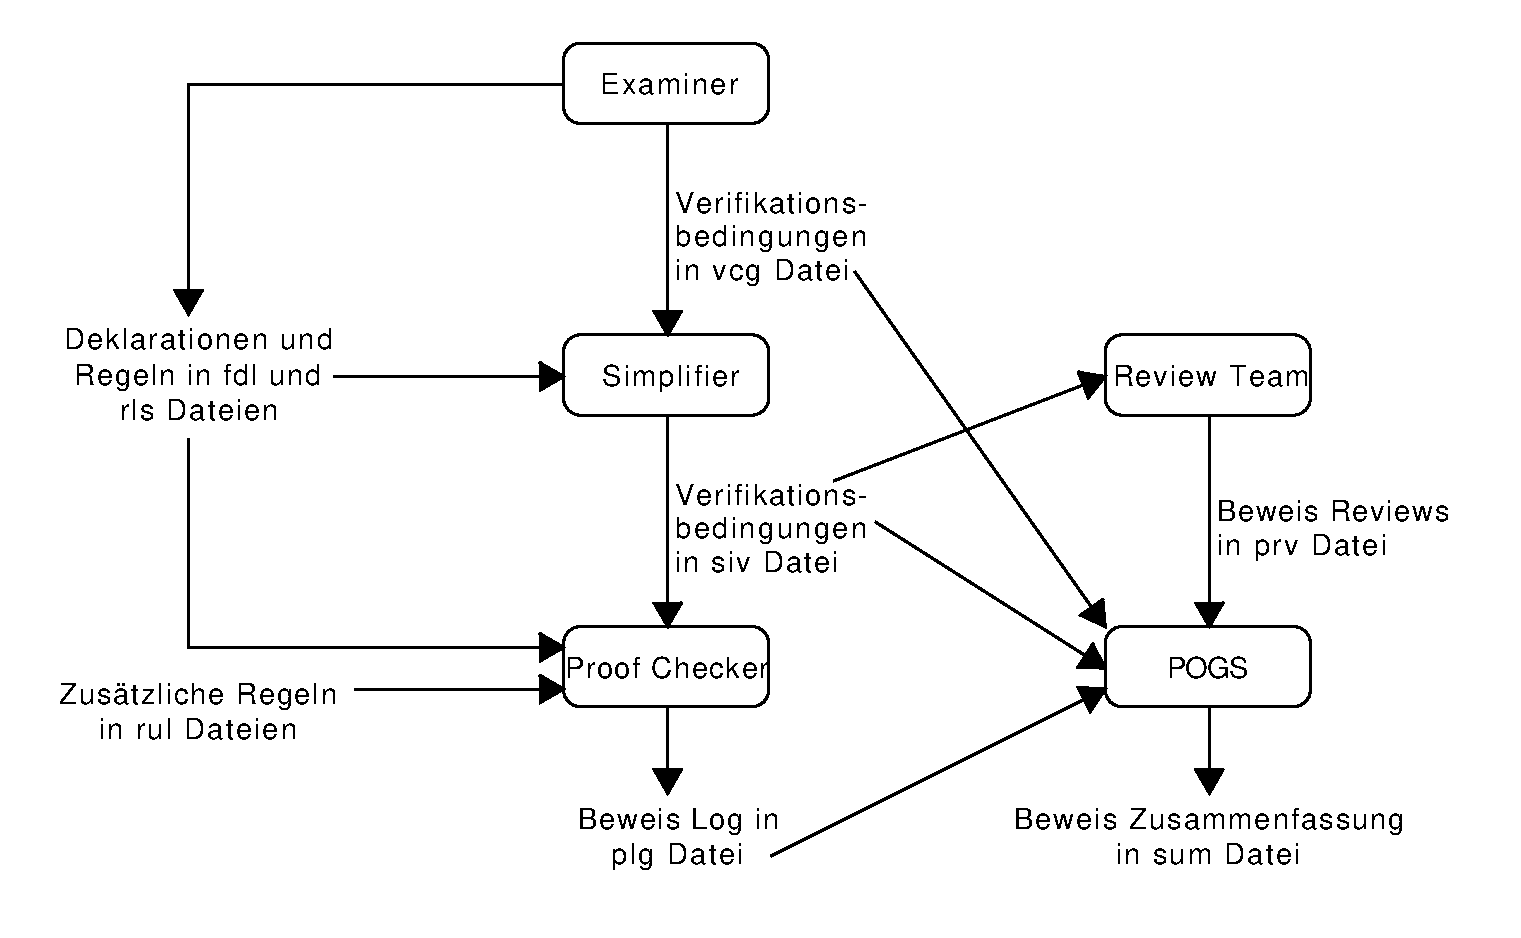
\includegraphics[width=\textwidth{}]{images/ProofProcess.pdf}
\label{fig:proofProcess}
\caption{Der gesamte Beweisprozess}
\end{figure}
Theorie hinter beweisverfahren der quelle entnehmen

\subsection{Examiner}
\label{sec:examiner}
Das wichtigste Tool ist der SPARK Examiner, der es erlaubt Programme abhängig von ihrer Wichtigkeit auf drei Ebenen zu analysieren. Die niedrigste Stufe ist dabei die \textbf{Datenflussanalyse}. Hier wird überprüft, dass Parameter und globale Variablen korrekt genutzt, Variablen nicht vor einer Wertzuweisung gelesen werden, Werte nicht ungenutzt bleiben, usw. Die derives Annotation wird bei der Flow Analyse ignoeriert.
Diese spielen erst bei der \textbf{Informationsflussanalyse} eine Rolle, welche die Norm für die meißten Programme darstellt. Es wird eine Datenflussanalyse durchgeführt und weiterhin wird die derives Annotation ausgewertet. Dadurch wird erkannt, wenn Variablen und Parameter korrekt genutzt werden. Da nur die statischen semantischen Beziehungen betrachtet werden und nicht dynamische Werte, wird diese Analyse auch manchmal flache Verfifikation genannt.
Bei sehr kritischer Software kommen Verifikationskonditionen, Flussanalyse und Beweis Annotationen zum Einsatz.

\subsubsection{Ausführungsreihenfolge}
Der Examiner überprüft ob Quelltexte, die mehrere Kompilierungseinheiten enthalten können, den Regeln von SPARK folgen. Dazu muss es, ähnlich wie beim Compiler, möglich sein auf andere Einheiten, die referenziert wurden, zuzugreifen. Dabei gibt es folgende Regeln:

\begin{itemize}
\item Um den Package Body zu analysieren braucht der Examiner Zugriff auf die Package Spezifikation und die Spezifikation privater Kinder.
\item Um eine Paket Spezifikation oder ein main Unterprogramm, dass von anderen Paketen erbt, zu analysieren braucht der Examiner Zugriff auf die Spezifikationen der anderen Pakete und deren Überklassen.
\item Zur Analyse einer Kind Einheit (child unit) wird die Elternspezifikation benötigt.
\item Für Subunits ist der Zugriff auf die einschließende Unit nötig. 
\end{itemize}
Der Examiner wird über die Komandozeile mit den zu analysierenden Dateien aufgerufen. Er analysiert die Einzeldateien in der gegebenen Reihenfolge. Dabei ist darauf zu achten, dass die Reihenfolge richtig gewählt ist und Abhängigkeiten entsprechend aufgelöst werden können. Für jede Quelldatei wird ein Listing File mit Fehler- und Warnmeldungen und einem Report der Analyse angelegt.
Mit folgendem Aufruf kann solch eine Analyse gestartet werden:
\begin{verbatim}
spark stack.ads stack.adb gobtween.ads gobtween.adb main.ada
\end{verbatim}
Es werden ein Report \texttt{spark.rep} und die drei Listing Dateien \texttt{main.lst},  
\texttt{stack.lst}, \texttt{gobtween.lst} erstellt.
Aufgrund der Abhängigkeiten müssen (im Gegensatz zur Kompilierung) bei einer Änderung alle Dateien neu vom Examiner betrachtet werden.

\subsubsection{Nachrichten}
Die Analyse des Examiner läuft in mehreren Schritten ab. Zunächst wird eine lexikographische und Syntaxanalyse durchgeführt. Dabei werden auchdie Abhängigkeiten aufgelöst. Die Ausgabe in Form von Fehler- und Warnmeldungen ähnelt der eines Compilers. In dieser Phase werden auch Inkonsistenzen in Bezug aud Annotationen aufgedeckt.
Interessanter wird es bei der Flussanalyse. Die Analyse wird in Unterprogrammblöcken ausgeführt.
Die Ausgaben haben folgende Form:
\begin{verbatim}
+++		Flow analysis of subprogramm Push performed: no errors found.
\end{verbatim}

Wurde das Package \texttt{The\_Stack} initialisiert kommt die folgende Meldung:

\begin{verbatim}
+++		Flow analysis of package initialization performed: no errors found.
\end{verbatim}

Einige Beispiele für Fehlernachrichten:
\begin{verbatim}
!!! (1)	Flow Error : 10 : Assignment to A is ineffective.
!!! (2) Flow Error : 33 : The variable A is neither referenced nor exported.
\end{verbatim}

\subsubsection{Optionen}
Wir beschränken uns an dieser Stelle auf eine tabellarische Übersicht der wichtigsten Optionen, da eine Beschreibung aller Optionen den Rahmen der Arbeit sprengen würde.

\begin{footnotesize}
\begin{table}[h!]
\centering
\caption{Zusammenfassung der wichtigsten Optionen des Examiners.}
\label{my-label}
\begin{tabular}{|l|l|l|l|}
\hline
{\it Option}          & {\it Kürzel}     & {\it Default} & {\it Beschreibung}                     \\ \hline
Analyse Optionen:     &                  &               &                                        \\
syntax\_check         & /sy              &               & nur Syntax Check                       \\
flow\_analysis        & /fl=type         & information   & Informations- oder Datenflussanalyse   \\
                      &                  &               & kann data oder information sein.       \\
                      &                  &               & Abkürzung:/fl=d oder /fl=i             \\
vcs                   & /vc              &               & erzeugt Verifikationsbedingungen       \\
rtc                   & /rt              &               & vcs und Laufzeitchecks                 \\
exp\_checks           & /e               &               & rtc und Overflow Checks                \\ \hline
Dateioptionen:        &                  &               &                                        \\
report\_file          & /r=file\_spec    & spark.rep     & Name der Reportdatei                   \\
listing\_extension    & /l=file\_type    & list          & Listing Dateiendung                    \\
html                  & /ht              &               & erzeugt html                           \\
index\_file           & /i=file\_spec    &               & Identifiziert Indexdatei               \\
warning\_file         & /w=file\_spec    &               & Identifiziert Warnungsdatei            \\
config\_file          & /conf=file\_spec &               & Identifiziert Zielkonfig Datei         \\ \hline
Andere Optionen:      &                  &               &                                        \\
annotation\_character & /an=character    & \#            & überschreibt normales --\#             \\
statistics            & /st              &               & erzeugt Nutzerstatistik                \\
plain\_output         & /pl              &               & unterdrückt Datum, etc. \\
fdl\_identifiers      & /fd              & reserved      & fdl Zeichen sind reserviert            \\
nofdl\_identifiers    & /nofd            &               & fdl Zeichen nicht reserviert           \\
help                  & /he              &               & Fasst Optionen zusammen                \\ \hline
\end{tabular}
\end{table}
\end{footnotesize}



\subsubsection{Metadateien und Indexdateien}
Ab einer gewissen Projektgröße wird es zu umständlich alle Dateinamen für den Examiner anzugeben. Hier schaffen Meta- und Indexdateiene Abhilfe.

Eine \textbf{Metadatei} ist eine simple Textdatei, die pro Zeile den Namen einer Quelldatei enthält. Ein Beispiel ist die Datei \texttt{meta.smf}

\begin{verbatim}
--metafile
stack.ads
stack.adb
gobtween.ads
gobtween.adb
main.ada
\end{verbatim}

Der Aufruf wird damit verkürzt auf:

\begin{verbatim}
spark @main.smf
\end{verbatim}

Es ist möglich eine Hierarchie von Metadateien zu erzeugen. Sind andere Metadateien enthalten, so müssen diese das Prefix @ haben. Das vorherige Beispiel könnte mit einer \texttt{stack.smf} und einer \texttt{gobtween.smf} umstrukturiert werden zu

\begin{verbatim}
--nested metafile
@stack.smf
@gobtween.smf
main.ada
\end{verbatim}

Mit dem Zusatz \texttt{\/l=} kann explizit der Name für die Listing Ausgabe angegeben werden.

Eine \textbf{Indexdatei} assoziiert Kompilierungseinheiten mit den Dateien, die sie enthalten. Für das bekannte Beispiel könnte diese Datei folgenden Inhalt haben:

\begin{verbatim}
The_Stack	specification	is in	stack.ads
The_Stack	body			is in	stack.adb
Go_Between	specification	is in	gobtween.ads
Go_Between	body			is in	gobtween.adb
Main		main_program	is in	main.ada
\end{verbatim}

Das main Programm kann dann mit dem Kommando
\begin{verbatim}
spark /index_file=example.idx main.ada
\end{verbatim}
analysiert werden. Bei diesem Aufruf wird nur das Listing für \texttt{main} erstellt und alle Informationen über Fehler in den Abhängigkeiten sind im Report zu finden.

Die Syntaxregeln für eine Indexdatei sind:
\begin{itemize}[label={}]
\item index\_file ::= [super\_index] {index\_entry}
\item super\_index ::= superindex is in file\_spec
\item index\_entry ::= file\_entry $|$ component\_entry
\item file\_entry ::= unit\_name entry\_type is in file\_spec
\item entry\_type ::= auxindex $|$ main\_program $|$ specification $|$ body $|$ subunit
\item unit\_name ::= Ada\_unit\_name
\item component\_entry ::= unit\_name components are unit\_name {, unit\_name}
\end{itemize}

Ein Superindex wird durchsucht, wenn die Suche in regulären Indexdateien fehlschlägt. Damit können Indexe hierarchisch strukturiert werden. Gibt es mehrere Dateien, die in mehreren Projekten immer wieder benötigt werden, so können diese beispielsweise in einer Datei \texttt{library.idx} abgelegt werden.

\begin{verbatim}
Spark_IO specification is in sparkio.ads
Spark_IO body is in sparkio.adb
Spark_Elementary_Functions specification is in sparkef.ads
...
\end{verbatim}

Der index eines Projekts kann dann anfangen mit:

\begin{verbatim}
superindex is in library.idx
...
\end{verbatim}

Da es möglich ist Dateien in subunits zu unterteilen, können diese natürlich auch in Indexdateien angegeben werden.

\begin{verbatim}
...
The_Stack body is in stacksep.adb
The_Stack.Push subunit is in push.adb
The_Stack.Pop subunit is in pop.adb
...
\end{verbatim}

Ein alternativer Ansatz ist es eine extra Indexdatei für \texttt{The\_Stack} anzulegen (z.B. \texttt{stackaux.idx}).

\begin{verbatim}
The_Stack body is in stacksep.adb
The_Stack.Push subunit is in push.adb
The_Stack.Pop subunit is in pop.adb
\end{verbatim}

Die Hauptdatei sieht dann entsprechend so aus:

\begin{verbatim}
The_Stack specification is in stack.ads
The_Stack auxindex is in stackaux.idx
...
\end{verbatim}

\texttt{Push} kann dann mit dem Aufruf

\begin{verbatim}
spark /i=main.idxpush.adb
\end{verbatim}

analysiert werden.
Der Examiner stellt zunächst fest, dass er den body von \texttt{The\_Stack} benötigt. Dieser kann im Index nicht gefunden werden und daraufhin wird der Auxiliary file durchsucht.

Es wäre weiterhin möglich \texttt{main.idx} zum Superindex zu machen und die anderen Angaben in \texttt{stackadb.idx} zu machen. Generell gibt es scheinbar keine Konventionen für das Anlegen der Indexdateien und man sollte sich nach der Struktur des jeweiligen Projektes richten. Schleifenabhängigkeiten sind zu vermeiden, da diese nicht vor dem Aufruf entdeckt werden und somit zu einer Dauerschleife führen.

\subsubsection{Beispiel Report}
Das hier gezeigte Report Beispiel zeigt die genutzen Optionen und Dateien und fasst alle Fehler und Warnungen zusammen. In der Spezifikation von Spark\_IO gibt es zwei Warnungen. Die erste bezieht sich auf die with clause für Ada.Text\_IO. Die Warnung kommt zustande, da die Spezifikation dem Examiner nicht zur Verfügung stand.
Die zweite Warnung zeigt, dass die privaten Teile von Spark\_IO versteckt sind.

Es ist möglich Warnungen zu unterdrücken indem eine Kontrolldatei für die Warnungen mitgegeben wird. Diese hat die Endung \texttt{.wrn} und enthält die Typen der zu unterdrückenden Warnungen.

\begin{verbatim}
**********************************************************************
                     Report of SPARK Examination
     SPARK95 Examiner with VC and RTC Generator Release 6.3 / 11.02
                        Demonstration Version
**********************************************************************

     DATE : 16-NOV-2002 13:45:12.26

Options:
    index_file=DIALOG.IDX
    nowarning_file
    notarget_compiler_data
    noconfig_file
    source_extension=ADA
    listing_extension=LST
    nodictionary
    report_file=SPARK.REP
    no_html
    nostatistics
    fdl_identifiers
    flow_analysis=information
    ada95
    annotation_character=#
    profile=sequential

Selected files:
    DIALOG.ADA

Index Filename(s) used were:
    C:\PRAXIS\DIALOG.IDX
    C:\PRAXIS\INVENT.IDX
    C:\PRAXIS\COMMON.IDX

No Meta Files used

Full warning reporting selected

Source Filename(s) used were:
    C:\PRAXIS\DIALOG.ADA
    C:\PRAXIS\INVENT.ADS
    C:\PRAXIS\SPARKIO.ADS

Source Filename: C:\PRAXIS\INVENT.ADS
No Listing File

    Unit name: Inventory
    Unit type: package specification
    Unit has been analysed, any errors are listed below.

1 error(s) or warning(s)
Line
  37 end Inventory;
         ^1
--- ( 1) Warning:394:Variables of Type
         Inventories cannot be initialized using the
         facilities of this package.

Source Filename: C:\PRAXIS\SPARKIO.ADS
No Listing File

    Unit name: Spark_IO
    Unit type: package specification
    Unit has been analysed, any errors are listed below.

2 error(s) or warning(s)

Line
  24 with Ada.Text_IO;
          ^1
--- ( 1) Warning:1:The identifier Ada is
         either undeclared or not visible at this point.

 308 end Spark_IO;

--- ( 2) Warning:10:The private part of
         package Spark_IO is hidden - hidden text is 
         ignored by the SPARK examiner.

Source Filename: C:\PRAXIS\DIALOG.ADA
Listing Filename: C:\PRAXIS\DIALOG.LST

    Unit name: Dialogue
    Unit type: main program
    Unit has been analysed, any errors are listed below.

2 error(s) or warning(s)

Line
  52 while True loop
           ^1
!!! ( 1) Flow Error:40:Exit condition is stable, of
         index 0.

  72 end Dialogue;

--- ( 2) Warning:400:Variable Found is declared
         but not used.

--End of file-------------------------------------------
\end{verbatim}

\subsubsection{Beweis Optionen}
Der Examiner erstellt neben den Listings und Reports auch Dateien mit Pfadfunktionen und Verifizierungsbedingungen.

Die Optionen \texttt{/vc}, \texttt{/rtc} und \texttt{/exp} erzeugen Verifikationsbedingungen auf verschiedenen Ebenen. Die Option \texttt{/vc} erzeugt die üblichen Bedingungen und weitere für run-time Checks. Dabei wird eine Datei mit der Endung \texttt{.vcg} erstellt.
Es werden weitere Dateien erstellt, wie in Abbildung ~\ref{fig:examinerFiles} gezeigt wird.

\begin{figure}[h!]
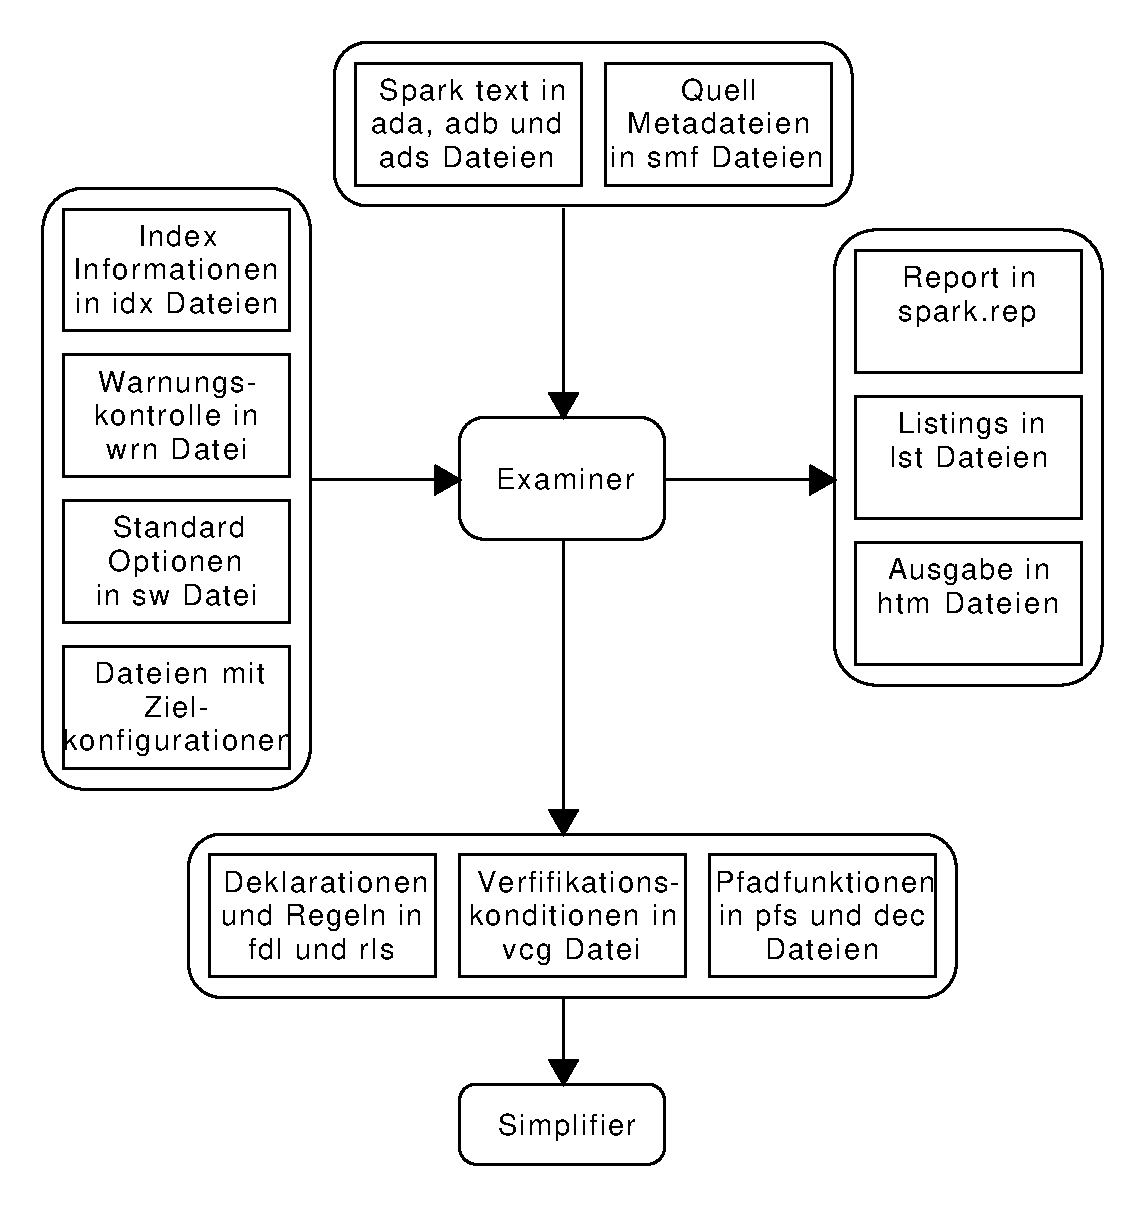
\includegraphics[width=\textwidth{}]{images/examinerFiles.pdf}
\label{fig:examinerFiles}
\caption{Der Examiner mit den zugehörigen Dateien.}
\end{figure}

\subsection{Simplifier}
Der Examiner erzeugt für jedes analysierte Unterprogramm eine \texttt{vcg} Datei mit rohen Verifikationsbedingungen. Diese sind in einer Baumstruktur angeordnet. Weiterhin werden \texttt{fdl} und \texttt{rls} Dateien erstellt, die Informationen zu den Objekttypen und deren Regeln zur Manipulation enthalten. Diese Dateien bilden den Input für den \textbf{Simplifier}.
Der Aufruf des Simplifiers erfolgt ebenfalls in der Konsole und ist einfacher zu Handhaben als der Examiner, da es weitaus weniger Konfigurationsbefehle gibt. Für eine Datei \texttt{example.vcg} mit den entsprechenden \texttt{fdl} und \texttt{rls} Dateien im selben Ordner ist der Aufruf

\begin{verbatim}
spadesimp example
\end{verbatim}

Die vereinfachten Verifikationsbedingungen werden in einer \texttt{siv} Datei gespeichert. Ein Log wird in einer \texttt{slg} Datei angelegt.
Mit dem Aufruf
\begin{verbatim}
sparksimp
\end{verbatim}
werden im aktuellen Verzeichnis und allen Unterverzeichnissen automatisch alle Dateien bearbeitet.

Der Simplifier kann auch Pfadfunktionen vereinfachen, dazu muss beim Aufruf einer \texttt{pfs} Datei die Dateiendungmit angegeben werden. 

\subsection{Proof Checker}
Die Arbeit des Proof Checkers verläuft nicht komplett automatisch, da dies den Rahmen des möglichen sprengen würde. Das Tool ist sehr komplex und mächtig, deswegen können hier nur die Grundzüge erläutert werden.

Ein wichtiger Aspekt des Proof Checkers ist das Logging. Im Log enthalten sind die Hypothesen und Regeln, die füreinen Beweis genutzt wurden und eine Übersicht über die noch zu erledigenden Beweise.
Der Proof Checker wendet einen Satz von Regeln und Strategien an um seine Arbeit zu verrichten. Exemplarisch seien hier einige Regeln genannt. Es gibt simple arithmetisiche Regeln.
\begin{verbatim}
arith(3): X + 0 may_be_replaced_by X.
assoc(4): A*(B*C) may_be_replaced_by (A*B)*C.
distrib(1): A*(B+C) & A*B + A*C are_interchangeable.
\end{verbatim} 
Weiterhin können Regeln auch Bedingungen haben, wie im folgenden Beispiel:
\begin{verbatim}
arith(12): (X/Y)*Y may_be_replaced_by X if [Y<>0].
\end{verbatim}
Es können auch Fakten aus anderen Fakten abgeleitet werden:
\begin{verbatim}
odd(5): odd(X) may_be_deduced_from [odd(-X)].
\end{verbatim}

In der gleichen Datei können beliebig viele Regeln jeder Art gespeichert werden.
Bei der deklaration eigener Regeln ist undbedingt auf deren Korrektheit zu achten, da sonst das ganze Konzept des Proof Checkers ad absurdum geführt würde.

\subsection{Proof Obligation Summarizer}
Nachdem der Simplifier seine Arbeit verrichtet hat, kann der Proof Obligation Summarizer(\textbf{POGS}) mit
\begin{verbatim}
pogs
\end{verbatim}
aufgerufen werden. Das aktuelle Verzeichnis wird dann nach relevanten Dateien durchsucht. POGS erstellt daraus eine Zusammenfassung in einer \texttt{sum} Datei. Diese enthält eine komplette Analyse der Situation. Gezeigt werden die Verifikationsbedingungen, die eliminiert bzw. bewiesen wurden, wie sie bewiesen wurden und was noch bewiesen werden muss.

%======================================================================
%   Literaturverzeichnis
%======================================================================
\renewcommand{\baselinestretch}{1.13}\normalsize
\markboth{BIBLIOGRAPHY}{BIBLIOGRAPHY}
\renewcommand{\bibname}{BIBLIOGRAPHY}
\bibliographystyle{plaindin}
\selectlanguage{ngerman}
\bibliography{literatur}
\cleardoublepage

%======================================================================
%   Selbstständigkeitserklärung
%======================================================================
\selectlanguage{ngerman}
\section*{Selbstständigkeitserklärung}
\thispagestyle{empty} Hiermit erklären wir, dass wir die vorliegende
Arbeit selbstständig angefertigt, nicht anderweitig zu
Prüfungszwecken vorgelegt und keine anderen als die angegebenen
Hilfsmittel verwendet haben. Sämtliche wissentlich verwendete
Textausschnitte, Zitate oder Inhalte anderer Verfasser
wurden ausdrücklich als solche gekennzeichnet.%\\[2ex]


\vspace{1cm}\noindent
--------------------------------- \newline
\vspace{1cm}\noindent
--------------------------------- \newline


Görlitz, den XXXXX

\end{document}